\section{Socket-Schnittstelle}

Die \textbf{Socket-Schnittstelle} ermöglicht die Kommunikation von verteilten Client-Server-Anwendungen untereinander.

\begin{tcolorbox}[enlarge top by=0.5cm,enlarge bottom by=0.5cm]
Die Socket-Schnittstelle stellt eine Schnittstelle zwischen \textbf{Schicht 4} (Transportschicht) und \textbf{Schicht 5} (Anwendungsschicht) dar.
\end{tcolorbox}

\subsection{Socket-Schnittstelle zu UDP}

Eine Schnittstelle zu \textbf{UDP} ist relativ einfach zu realisieren, da hier keine Operationen für den Verbindungsauf- und -abbau nötig sind $\rightarrow$ es sind nur Operationen für das Senden und Empfangen notwendig.\\

\noindent
Bei der Erzeugung eines \textbf{Sockets} kann eine Portnummer angegeben werden, für gesendete Nachrichten ist das dann die \textbf{Quellportnummer} der Nachricht.\\
Der Socket empfängt nur Nachrichten, die an diesen Port adressiert wurden.\\

\noindent
Bei \textbf{Client/Server-Anwendungen} geht die Initiative vom Client aus, der eine Anfrage an einen Server schickt.\\
Der Server antwortet an die in der Nachricht enthaltenen IP-Adresse und Quellportnummer.

\begin{tcolorbox}[enlarge top by=0.5cm,enlarge bottom by=0.5cm]
I.d.R verwendet ein Client eine beliebige freie Portnummer.\\

\noindent
Dienste laufen auf Servern auf wohlbekannten Portnummern, bspw. ``https`` auf Port $443$\footnote{
s. a. ``Hypertext Transfer Protocol Secure``: \url{https://de.wikipedia.org/wiki/Hypertext_Transfer_Protocol_Secure} - abgerufen 30.01.2024
}.\\
Ein Server, der unter einer bestimmten Portnummer laufen soll, kann nur gestartet werden, wenn die Portnummer nicht schon belegt ist.
\end{tcolorbox}\\

\newpage
\noindent
Beispiel für eine Programmstruktur für eine Kommunikation zwischen UDP-Client und -Server:
\begin{minted}[mathescape,

    numbersep=5pt,
    gobble=2,
    frame=none,
    framesep=2mm]{java}
    // UDP Client
    c = ErzeugeUDPSocket();
    while (beliebig) {
        sende Nachricht über Socket c an ServerAdresse/Portnummer;
        warte auf Nachricht an Socket c;
        tue etwas mit der Nachricht;
    }

    // UDP Server
    s = ErzeugeUDPSocketAnPort(port);
    while (beliebig) {
        warte auf Nachricht von Client an Socket s;
        analysiere die Nachricht;
        führe Aktion aus;
        schicke über s Antwort an die Adresse/Portnummer der Nachricht;
    }
\end{minted}

\begin{tcolorbox}[enlarge top by=0.5cm,enlarge bottom by=0.5cm]
    Die Portnummern für \textbf{TCP} und \textbf{UDP} existieren unabhängig voneinander: Ist ein Port $n$ für TCP reserviert, kann die gleiche Portnummer trotzdem für UDP verwendet werden.
\end{tcolorbox}

\subsection{Socket-Schnittstelle zu TCP}

Die Besonderheit bei TCP ist, dass der Server auf einen Port auf eine Anfrage (über einen Socket) wartet, und dann mit dem Client die Kommunikation über einen neuen Socket realisiert (s. Abbildung~\ref{fig:tcpsockets}).\\

\begin{figure}
    \centering
    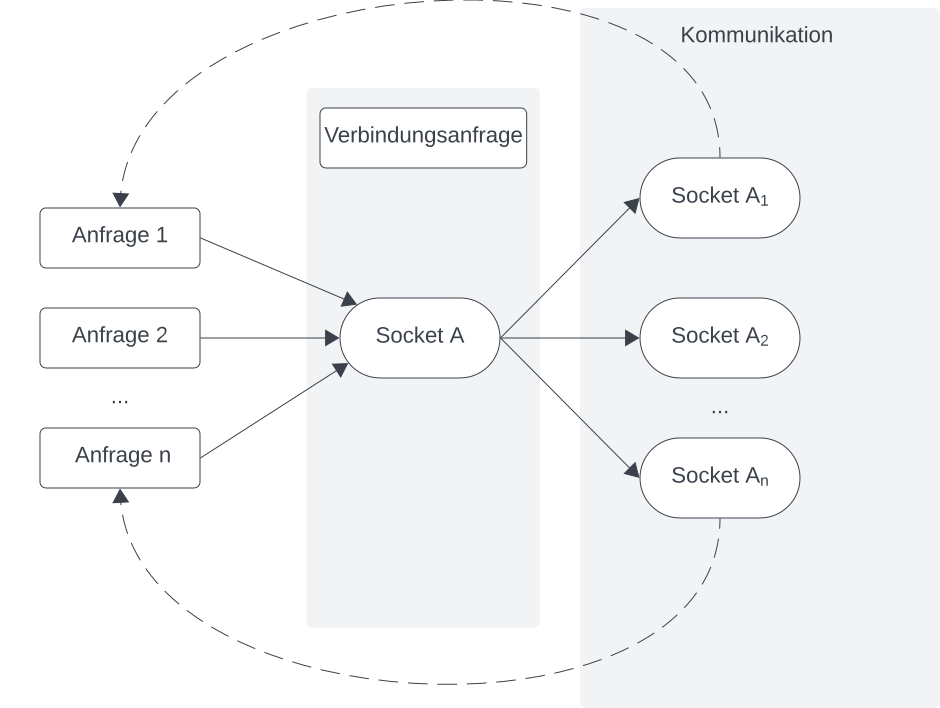
\includegraphics[scale=0.5]{chapters/fopt5/img/sockets/tcpsockets}
    \caption{Von einem TCP-Socket angenommene Verbingungsanfragen führen zu neuen Sockets, die letztendlich für die Kommunikation mit den Clients verantwortlich sind.
    Nach Verbindungsabbruch werden diese Sockets verworfen, der Socket zur Verbindungsannahme wird weiterverwendet(Quelle: eigene)}
    \label{fig:tcpsockets}
\end{figure}



\noindent
$\rightarrow$ für einen Port kann es somit mehrere Sockets geben.\\


\noindent
Beispiel für eine Programmstruktur für eine Kommunikation zwischen UDP-Client und -Server:
\begin{minted}[mathescape,
    numbersep=5pt,
    gobble=2,
    frame=none,
    framesep=2mm]{java}
    // TCP Client
    c = ErzeugeTCPSocket();
    baue über c eine Verbindung zu ServerAdresse/Portnummer auf;
    /* c ist blockiert, bis Timeout abgelaufen oder Anfrage angenommen */
    while (beliebig) {
        sende Nachricht über Socket c;
        warte auf Nachricht an Socket c;
        tue etwas mit der Nachricht;
    }
    schliesse die Verbindung über c;

    // TCP Server
    s = ErzeugeTCPSocketAnPort(port);
    while (beliebig) {
        warte auf Verbindungsanfrage an s und erstelle
        neuen Socket q bei neuer Verbindung;

        while (Verbindung besteht) {
            warte auf Nachricht von Client an Socket q
            wenn nachricht da ist {
                analysiere die Nachricht;
                führe Aktion aus;
                schicke über q Antwort an die Adresse/Portnummer
                der Nachricht;
            } ansonsten nach timeout oder verbindungsabbruch {
                schliesse Verbindung über q;
                verlasse die innere schleife und warte auf
                neue verbindung;
            }

        }
    }
\end{minted}\\

\noindent
Es gibt bei \textbf{TCP} höchstens eine Verbindung von einem Port auf einem Rechner zu einem anderen Port auf einen anderen Rechner, aber es können mehrere Verbindungen von einem Port zu unterschiedlichen Ports des Zielrechners existieren, bzw. es kann ein Rechner mehrere Verbindungen zu einem bestimmten Port auf einem unterschiedlichen Zielrechner erstellen (s. Abbildung~\ref{fig:tcpconnections}).


\begin{figure}
    \centering
    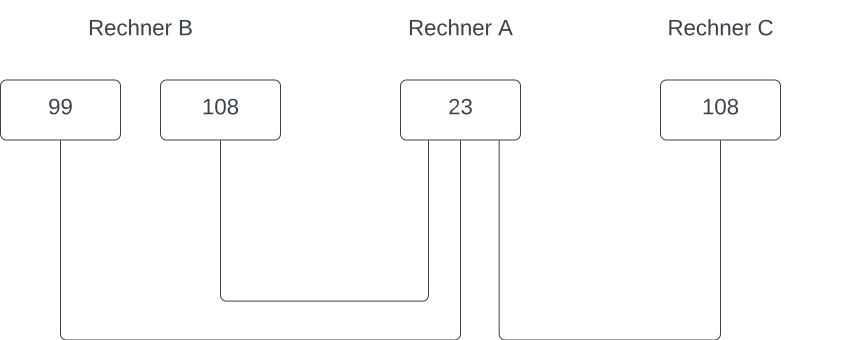
\includegraphics[scale=0.5]{chapters/fopt5/img/sockets/tcpconnections}
    \caption[fontsize=\small]{Rechner $A$ bedient zweimal dieselbe Portnummer $108$ auf zwei unterschiedlichen Rechnern $B$ und $C$, von Port $23$ aus. Gleichzeitig wird Port $99$ von Rechner $B$ von Rechner $A$ bedient. (Quelle: in Anlehnung an \cite[265, Bild 5.3]{Oec22})}
    \label{fig:tcpconnections}
\end{figure}


\subsection{Socket-Schnittstelle für Java}

Die Java-Klassenbibliothek enthält u.a. im Package \code{java.net} Implementierung zur Realisierung von Socket-Kommunikation.\\

\noindent
\code{InetAddress} ist eine Klasse zur Handhabung von von Rechnernamen / IP-Adressen.\\

\noindent
\code{DatagramPacket} und \code{DatagramSocket} werden zur \textbf{UDP}-Kommunikation verwendet.\\

\noindent
\code{Socket} und \code{ServerSocket} werden zur \textbf{TCP}-Kommunikation benötigt.


\section{Kommunikation über UDP mit Java Sockets}

\code{DatagramPacket} wird mit der IP-Adresse und Portnummer des Partners konfiguriert $\rightarrow$ für zu sendende Pakete ist das die Ziel-Adresse und Ziel-Portnummer, für empfangene Pakete ist das die Quelladresse und Quell-Portnummer.\\

\noindent
Ein \code{DatagramPacket} repräsentiert Daten in Form eines Feldes des Typs \code{byte} und einer Länge, die höchstens so groß sein kann wie die Feldlänge - ist die Länge kleiner als die Feldlänge, wurde nur die angegebene Länge als relevant betrachtet.\\

\noindent
Server verwenden für die Kommunikation bei der Erzeugung von \code{DatagramSocket} i.d.R. eine feste Portnummer, auf der der Service laufen soll.\\
Clients verwenden i.d.R. den parameterlosen Konstruktor, ein freier Port wird dann zugeteilt.

\begin{minted}[mathescape,
    numbersep=5pt,
    gobble=2,
    frame=none,
    framesep=2mm]{java}
    public class DatagramPacket {
        public DatagramPacket(byte[] buf, int length) {...}
        public DatagramPacket(
            byte[] buf, int length, InetAddress address, int port) {...}
        ...
    }

    public class DatagramSocket implements Closeable {
        public DatagramSocket() throws SocketExcpetion {...}
        public DatagramSocket(int port) throws SocketExcpetion {...}
        public send(DatagramPacket p) throws IOExcpetion {...}
        public receive(DatagramPacket p) throws IOExcpetion {...}
        ...
    }
\end{minted}\\

\noindent
Die Methode \code{receive()} eines Sockets ist \texbf{blocking}, es wird so lange gewartet, bis eine Nachricht eintrifft, oder ein durch \code{setSoTimeout(int timeout)} angegebener Timeout eintritt.\\

\noindent
Mit \textbf{try-with-resources}\footnote{
    ``The try-with-resources Statement``: \url{https://docs.oracle.com/javase/tutorial/essential/exceptions/tryResourceClose.html} - abgerufen 31.01.2024
} kann ein Socket automatisch geschlossen werden.

\begin{tcolorbox}[enlarge top by=0.5cm,enlarge bottom by=0.5cm]
Ein Objekt, dessen Klasse \code{AutoCloseable} implementiert, kann als \textit{Resource} für das \textit{try-with-resource}-Statement genutzt werden.
Das schliesst auch Objekte ein, deren Klasse \code{Closeable} implementiert, da \code{Closeable} von \code{AutoCloseable} abgeleitet ist.\\

\noindent
Wenn \code{AutoCloseable}-Objekte weder mit \textbf{try-with-resources} noch mit \code{close} verwendet werden, gibt der Compiler seit Java 7 eine Warnung aus.\\

\noindent
Ein \code{try-with-resources}-Statement kommt ohne \code{catch}-Block aus.\\
Wenn die Konstruktoren der erzeugten Objekte eine Exception werfen, sollte das in der Methoden-Signatur angegeben werden, oder ein \code{catch}-Block sollte verwendet werden.
\end{tcolorbox}

\begin{minted}[mathescape,
    numbersep=5pt,
    gobble=2,
    frame=none,
    framesep=2mm]{java}
    try (DatagramSocket updSocket = new DatagramSocket(1234);
     PrintWriter pw = new PrintWriter("foo.txt");) {
        ...
    } catch (SocketException | FileNotFoundException e) {
        ...
    }
\end{minted}\\

\section{Multicast-Kommunikation mit Java-Sockets}
Mittels der Klasse \code{MulticastSocket} (abgeleitet von \code{DatagramSocket}) kann sich ein Socket mittels der Methode \code{joinGroup()} auf eine \textbf{Multicast-Adresse} aufschalten.\\
Der Socket erhält so jede Nachricht, die an diese Adresse geschickt wurde.\\
Mittels \code{leaveGroup()} schaltet sich der Socket von dem Nachrichtenempfang wieder ab.

\begin{tcolorbox}[enlarge top by=0.5cm,enlarge bottom by=0.5cm]
\textbf{IP-Multicast-Adressen} sind spezielle Adressen, mit denen mehr als ein Rechner angesprochen werden kann.\\
Für \textbf{IPv4} ist hierfür der Bereich $224.0.0.0 - 239.255.255.255$ reserviert\footnote{
s.a. ``Multicast address``: \url{https://en.wikipedia.org/wiki/Multicast_address} - abgerufen 31.01.2024
}.
\end{tcolorbox}

\noindent
Zum Senden von Nachrichten an eine Multicast-Adresse reicht ein \code{DatagramSocket}.\\
Will man aber einen \textbf{TTL}\footnote{\textit{Time-to-Live} - auch \textbf{hop limit} - wird verwendet, um ein Datenpaket mit einer max. Lebensdauer zu konfigurieren, was verhindern soll, dass Datenpakete unendlich lange in einem Netzwerk existieren. S. a. \url{https://en.wikipedia.org/wiki/Time_to_live} - abgerufen 31.01.2024}-Wert angeben, muss ein \code{MulticastSocket} verwendet werden.

\blockquote[{`DARPA INTERNET PROGRAM PROTOCOL SPECIFICATION`: \url{https://datatracker.ietf.org/doc/html/rfc791#section-1.4} - abgerufen 31.01.2024}]{
    The Time to Live is an indication of an upper bound on the lifetime of an internet datagram. It is set by the sender of the datagram and reduced at the points along the route where it is processed. If the time to live reaches zero before the internet datagram reaches its destination, the internet datagram is destroyed. The time to live can be thought of as a self destruct time limit.
}

\section{Kommunikation über TCP mit Java-Sockets}


Für \textbf{TCP}-Kommunikation werden in Java die Klassen \code{Socket} und \code{ServerSocket} eingesetzt.\\

\noindent
Der \textbf{Client} erzeugt ein \code{Socket}-Objekt unter Angabe der Adresse, zu der sich der Client verbinden möchte.\\

\noindent
Der \textbf{Server} nutzt die Klasse \code{ServerSocket}, der über \code{accept()} auf eingehende Verbindungen wartet.\\
Eine Verbindung wird von \code{accept()} über einen zurückgegebenen \code{Socket} signalisiert, der dann für die Kommunikation mit dem Client genutzt werden kann (s.a. Abbildung~\ref{fig:tcpsockets}).\\

\noindent
Eine \textbf{TCP}-Verbindung kann als zwei unidirektionale Verbindungen gesehen werden (Eingabe, Ausgabe).\\
$\rightarrow$ Es gibt deshalb nicht nur die Möglichkeit, mit \code{close()} der Klasse \code{java.net.Socket} die Verbindung komplett zu schließen, sondern es gibt darüber hinaus noch die Möglichkeiten, die Eingangs-/Ausgangsverbindungen getrennt voneinander zu schließen:


\begin{itemize}
    \item \code{shutdownInput()} $\rightarrow$ weiter senden, nicht mehr empfangen: ``Any data sent to the input stream side of the socket is acknowledged and then silently discarded.``\footnote{``Class Socket``: \url{https://docs.oracle.com/en/java/javase/21/docs/api/java.base/java/net/Socket.html#shutdownInput()} - abgerufen 31.01.2024
    }
    \item \code{shutdownOutput()} $\rightarrow$ weiter empfangen, nicht mehr senden.\footnote{``If you write to a socket output stream after invoking shutdownOutput() on the socket, the stream will throw an IOException.`` s. \url{https://docs.oracle.com/en/java/javase/21/docs/api/java.base/java/net/Socket.html#shutdownOutput()} - abgerufen 31.01.2024
    }
\end{itemize}

\noindent
\code{Socket} bietet keine Methoden zum Schreiben/Lesen {bzw.} Senden und Empfangen (vgl.~\cite[282]{Oec22}), stattdessen nutzt man die über \code{getInputStream()} / \code{getOutputStream()} zur Verfügung gestellten \textbf{Byteströme}.

\begin{tcolorbox}[enlarge top by=0.5cm,enlarge bottom by=0.5cm]
    \begin{itemize}
        \item \textbf{InputStream} / \textbf{OutputStream}: byteweise Ein-/Ausgabe
        \item \textbf{Reader} / \textbf{Writer}: zeichenweise Ein-/Ausgabe
    \end{itemize}
\end{tcolorbox}

\noindent
$\rightarrow$ über \textit{Adapter}/\textit{Dekorierer} kann man diese Byteströme direkt zum Lesen/Senden von \code{String}s nutzen.\\
I.d.R. sollte man hierfür Puffer nutzen die \textit{geflushed}\footnote{alles, was sich im Buffer befindet, wird an den darunterliegenden Ausgabestrom gesendet} werden, wenn sie voll sind, damit nicht für jedes einzelne Zeichen Betriebssystemaufrufe stattfinden müssen.\\

\noindent
Da \textbf{TCP} datenstromorientiert ist, kann man Trennzeichen zum Markieren von Nachrichtengrenzen nutzen.
Hierzu verwendet man in der Regel eine \textit{newline}, also \textbf{\textbackslash n}.

Beispiel für das Senden von Daten über einen Socket mittels eines \code{BufferedWriter}s\footnote{
    ``Class BufferedWriter``: \url{https://docs.oracle.com/en/java/javase/21/docs/api/java.base/java/io/BufferedWriter.html} - abgerufen 31.01.2024
}:
\begin{minted}[mathescape,
    numbersep=5pt,
    gobble=2,
    frame=none,
    framesep=2mm]{java}
    OutputStrean os = socket.getOutputStream();
    OutputStreamWriter ow = new OutputStreamWriter(os);
    BufferedWriter bw = new BufferedWriter(ow);
    ...
    bw.write("message");
    bw.newline();
    bw.flush();
\end{minted}\\

Beispiel für das Lesen von Daten über einen Socket mittels eines \code{BufferedReader}s\footnote{
    ``Class BufferedReader``: \url{https://docs.oracle.com/en/java/javase/21/docs/api/java.base/java/io/BufferedReader.html} - abgerufen 31.01.2024
}:
\begin{minted}[mathescape,
    numbersep=5pt,
    gobble=2,
    frame=none,
    framesep=2mm]{java}
    InputStream is = socket.getInputStream();
    InputStreamReader ir = new InputStreamReader(is);
    BufferedReader bw = new BufferedReader(ir);
    ...
    String message = br.readLine();
\end{minted}\\

\noindent
Das Ende eines Datenstroms wird durch den Rückgabewert \code{null} angezeigt (bei Dateioperationen {bspw.} als Ende der Datei; TCP-Verbindung: Client hat die Verbindung geschlossen usw.).

\begin{tcolorbox}[enlarge top by=0.5cm,enlarge bottom by=0.5cm]
    Das Lesen ist eine blockierende Operation.\\
    Das Schreiben von Daten mit anschliessendem \code{flush()} ist nicht blockierend.
    Sollte der Sender allerdings direkt nach dem Senden der Daten mithilfe einer Leseoperation auf die Antwort des Empfängers warten, ist auch diese Leseoperation blockierend und es kann erst wieder gesendet werden, nachdem der Aufrufer nicht mehr blockiert ist.
\end{tcolorbox}

\noindent
Solange ein \textbf{TCP}-Server\footnote{
 wie bspw in \cite[288, Listing 5.8]{Oec22} implementiert
} eine Verbindung mit einem Client aufrechterhält, kann keine andere Verbindung bearbeitet werden.\\
Ein \textbf{timeout} (Server wartet auf Nachricht von Client für $n$ Sekunden, danach schliesst er die Verbindung) ist hierzu eine (naive) Möglichkeit, Ressourcen freizumachen.

\subsection{Notizen zu den Übungen}
\subsection*{Übungen 5.3}
Sobald ein Server-Socket über Java gestartet wurde, können sich Clients zu diesem Server verbinden.\\
Dabei spiel es keine Rolle, ob der Server \code{accept()} zur Annahme neuer Verbindungen aufgerufen hat - sowohl die Clients als auch bereits gesendete Nachrichten werden vom OS bis zu einer gewissen Grenze gepuffert.\\
Sobald der Server dann \code{accept()} aufruft, wird ein Client aus dem Puffer genommen und die von ihm gesendeten Daten können gelesen werden (s. Skript FOPT5/6, S. 48).

\section{Sequenzielle und parallele Server}\label{sec:seqparserver}

Bei der Benutzung eines \textbf{TCP}-Servers wird nach der Annahme einer Verbindung nur von dieser Verbindung gelesen; die nächste Verbindung muss warten, bis die Verbindung geschlossen wird.\\
$\rightarrow$ Die Problematik kann umgangen werden, indem man für eine eingehende Verbindung einen neuen Thread startet, der mit dieser Verbindung arbeitet.\\

\noindent
$\rightarrow$ Möglichkeiten hierzu: \textbf{sequenzielle} durch \textbf{parallele} Implementierungen ersetzen.\\

\subsection*{Statische Parallelität}
Fixe Anzahl von Threads (``Verbindungen``) die von einem Server genutzt werden können.\\

$\rightarrow$ \textbf{Statische Parallelität} kann über ein Feld von Threads realisiert werden, oder einen \textbf{ThreadPool}\footnote{
``Thread Pools``: \url{https://docs.oracle.com/javase/tutorial/essential/concurrency/pools.html} - abgerufen 31.01.2024
}, bei dem \code{corePoolSize} $=$ \code{maxPoolSize} gilt (s.a.~\cite[146]{Oec22}).\\

\noindent
Statische Parallelität erlaubt es einem Server, eine \textit{fixe} Anzahl von Verbindungen gleichzeitig zu bedienen.\\
Hierbei wird ein Feld von Threads erstellt, wobei jeder Thread das \code{ServerSocket}-Objekt als Referenz übergeben bekommt.
In der \code{run()}-Methode wird dann über \code{accept()} in einer Endlosschleife auf eingehende Verbindungen gewartet, die dann so lange bedient werden, bis sich ein Client wieder abmeldet (oder eine andere Abbruchbedingung erfüllt ist, wie z.B. ein \code{SocketTimeout}).\\
Das sich ein Client abmeldet, bekommt man bspw. dadurch mit, dass \code{null} beim Lesen von einer Nachricht des Clients zurückgegeben wird (vgl. \cite[286]{Oec22}

Im Folgenden ein Implementierungsbeispiel für \textbf{Statische Parallelität}:
\begin{minted}[mathescape,
    linenos,
    numbersep=5pt,
    gobble=2,
    fontsize=\small,
    frame=lines,
    framesep=2mm]{java}
    class ServerThread extends Thread {
        private ServerSocket server;
        public ServerThread(ServerSocket sck) {
            this.server = sck;
            start();
        }
        public void run() {
            try (Socket socket = server.accept()) {
                while (true) {
                    // lesen & schreiben
                    // bei timeout oder exception Schleife verlassen
                }
            }
        }
    }

    class Server {
        private ServerThread[] serverThreads;

        public Server(int num) {
            serverThreads = new ServerThread[num];
            init();
        }
        private void init() {
            try {
                ServerSocket sck = new ServerSocket(8888));
            } catch (Exception e) {
                System.err.println(e);
                return;
            }
            for (int i = 0; i < clientThreads.length; i++) {
                serverThreads[i] = new ServerThread(sck);
            }
        }
    }
\end{minted}

\subsection*{Dynamische Parallelität}
Die Anzahl der Threads wachsen mit den eingehenden Verbindungen.\\

$\rightarrow$ Risiko eines DDoS ist erhöht, da viele Verbindungen einen Server beschäftigen können; je mehr Verbindungen angenommen werden, desto mehr Thread-Objekte werden erstellt, bis die Auslastung des Rechners zu groß wird.\\

\noindent
Bei \textbf{Dynamischer Parallelität} erzeugt der Server für jede Verbindung einen neuen Thread, der so lange läuft, bis der Client die Verbindung wieder trennt (oder eine andere Abbruchbedingung erfüllt ist, wie z.B. ein \code{SocketTimeout}).\\
Die Anzahl der Threads ändert sich dadurch laufend.


\subsection*{Mischform}
Fixe Anzahl von Threads, aber Anzahl wird erhöht, wenn die Auslastung hoch ist.\\

\noindent
Eine \textbf{Mischform} kann leicht realisiert werden, indem wieder ein \textbf{ThreadPool} verwendet wird, bei dem \code{maximumPoolSize} $>$ \code{corePoolSize} gilt und die \code{BlockingQueue}\footnote{ ``Interface BlockingQueue<E>``: \url{https://docs.oracle.com/en/java/javase/21/docs/api/java.base/java/util/concurrent/BlockingQueue.html} - abgerufen 31.01.2024; s.a.~\cite[146]{Oec22}} eine begrenzte Anzahl von Plätzen hat (darf nicht beliebig anwachsen).